%\vspace{-0.8em}
\subsection{Synthetic data experiments}
%\vspace{-0.8em}
We evaluated our algorithm using two synthetic datasets, reflecting all scenarios discussed in this paper. The metrics are abstention percentages (Abs. \%) and mistake counts (FP + FN), averaged over 1000 streams each with 2000 samples drawn from Normal distributions with random parameters, with $p=1-10^{-2}$ and $\alpha=10^{-3}$. Our comparisons against common thresholding baselines: $\tau^{30\%}$ for static thresholding, {\ttfamily DSpot} for dynamic thresholding, and {\ttfamily EQ} for empirical quantiles using online gradient descent, are presented in Table \ref{tab:synthetic}. Implementation details and additional experiments on Pareto distributions are in Appendix \ref{app:exp1}. These results confirm our algorithm's high accuracy, adaptability to distribution shifts, and effective learning from offline data, as outlined in Section 1's desiderata. Figure \ref{fig:synthetic} illustrates how our algorithm's abstention rates and errors grow over time, corroborating our theoretical results.
%theory that (1) our algorithm makes very little FP and FN, and (2) abstains are reduced significantly with the introduction of offline datasets.  evident in the low number of mistakes,
\begin{table}[h!]
    \centering
    \begin{tabular}{cc|c|c |c| c|c}
    \toprule
        shift & data &  & Ours &  $\tau^{30\%}$  & DSpot & EQ \\
        \midrule
        \midrule
         \multirow{2}{*}{x}  & \multirow{2}{*}{x}  &
         Abs. \%& $12.1$ \plusminus{1.4} & $30$ & $15$ & $0$ \\
          && FP+FN & $\mathbf{0}$ \plusminus{0}  & $5.3$ \plusminus{3.7} & $9.1$ \plusminus{3.6} & $3.9$ \plusminus{2.1}  \\
          \midrule
         \multirow{2}{*}{\checkmark}  & \multirow{2}{*}{x}  &  
         Abs. \%& $32.7$ \plusminus{9.1} & $30$ &  $15$ & $0$  \\
        && FP+FN & $\mathbf{5.2}$ \plusminus{1.3} &  $195$  \plusminus{71} & 225 \plusminus{95} & 219 \plusminus{71} \\
                    \midrule
        \multirow{2}{*}{x} & \multirow{2}{*}{\checkmark}  &  
        Abs. \% & 9.3 \plusminus{1.2} & $30$&  $15$ & $0$ \\
          && FP+FN  & $\mathbf{0}$ \plusminus{0} & $5.3$ \plusminus{3.7} & $9.1$ \plusminus{3.6} & $3.9$ \plusminus{2.1} \\
                    \midrule
        \multirow{2}{*}{\checkmark} & \multirow{2}{*}{\checkmark}  &  Abs. \% & $18.9$ \plusminus{4.1} &$30$ &  $15$ & $0$ \\
          && FP+FN & $\mathbf{2.0}$ \plusminus{1.5}  & 155 \plusminus{69} & 173 \plusminus{64} & 160 \plusminus{64} \\
         \bottomrule
    \end{tabular}
    \caption{Synthetic dataset results. We used Algorithm 1, 3, 4, 5 as ``ours" for the four settings respectively. Compared to baselines, we achieve significant less mistakes (FP+FN) with low abstain rate, especially in settings with shift.}
    \label{tab:synthetic}
\end{table}


\begin{figure}
\centering
% \begin{subfigure}{.45\columnwidth}
%   \centering
%   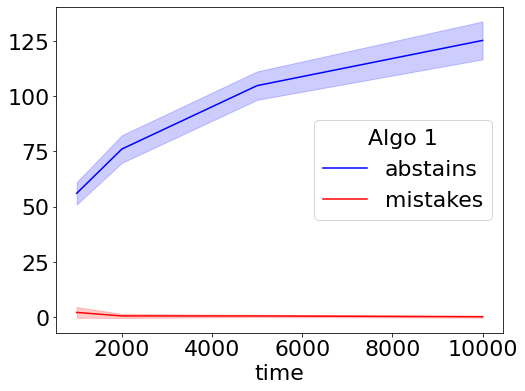
\includegraphics[width=\linewidth]{anomaly/figs/growth.png}
%   %\caption{Anomaly threshold set using a fixed cold-start period}
%   %\caption{}
%   %\label{fig:synthetic1}
% \end{subfigure}%
% \begin{subfigure}{.45\columnwidth}
%   \centering
%   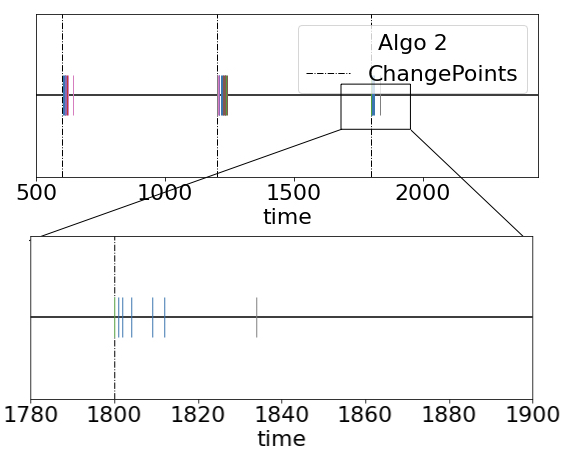
\includegraphics[width=\linewidth]{anomaly/figs/mistakes.jpeg}
%   %\caption{A subfigure}
%   %\caption{}
%   %\label{fig:synthetic2}
% \end{subfigure}
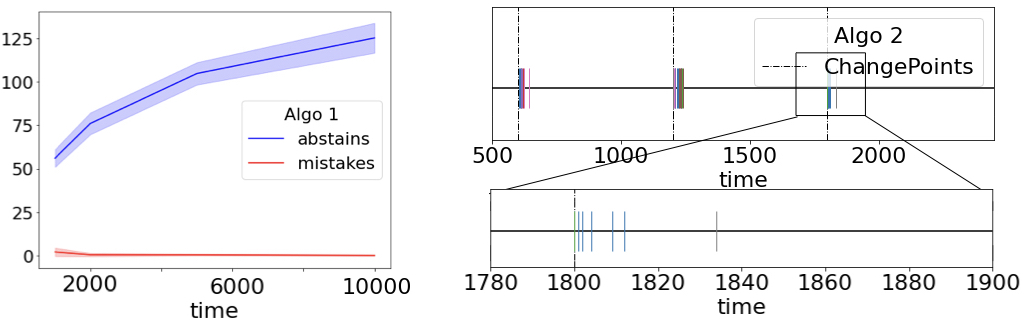
\includegraphics[width=0.95\linewidth]{anomaly/figs/exp1.jpeg}
\caption{\textit{Left:} algorithm 1, Abstains grows at $\gO(\sqrt{T})$. \textit{Right:}  algorithm 2, timestamp of mistakes in 10 random streams with aligned change points. Mistakes cluster right after change points, only as detection delay.}
\label{fig:synthetic}
\end{figure}

\subsection{MNIST anomaly detection}

We tested our algorithms on the MNIST dataset for one-class anomaly detection to demonstrate their real-world efficacy. We designated even digits as normal and odd digits as anomalous, and created data streams by sampling (e.g. Fig \ref{fig:mnist}). To show synergy of our thresholding algorithm with standard anomaly detection algorithms, we obtain anomaly scores from two models: convolutional autoencoder neural networks (NN) and isolation forests (IF), both trained on the normal class. With parameters set at $p = 0.99$ and $\alpha = 0.01$ for streams of 1000 samples, Table \ref{tab:mnist} illustrates our algorithm's improved performance over baselines.

\begin{table}[]
    \centering
    \begin{tabular}{l|c c||l | c c}
    \toprule
       Static  & abstains &  FP+FN  & Shift & abstains & FP+FN  \\
    \midrule
    $\tau^{30\%}$ & 327 \plusminus{0} & 12.7 \plusminus{0.9} &  $\tau^{30\%}$ & 670 \plusminus{0} & 91 \plusminus{8.0}\\
    DSpot & 150 \plusminus{0} & 78.1 \plusminus{2.5}  & DSpot & 150 \plusminus{0} & 129.5 \plusminus{10.2} \\
    IF+A1 & 172 \plusminus{16} & 17.6 \plusminus{5.3}  & IF+A3 & 190  \plusminus{39} & 75.7 \plusminus{18.9}\\
    NN+A1 & 133 \plusminus{4} & \textbf{3.9} \plusminus{0.7}  & NN+A3 & 339 \plusminus{12} & \textbf{9.3} \plusminus{2.1} \\
    NN+A5 & 89 \plusminus{6} & \textbf{2.1} \plusminus{0.2}  &  NN+A5 & 210 \plusminus{8} & \textbf{8.8} \plusminus{2.3} \\
    \bottomrule
    \end{tabular}
    \caption{One class MNIST result. We applied our algorithms (A as shorthand) to anomaly scores generated by Isolation Forest (IF) and neural networks (NN) and achieve much lower mistakes with moderate number of abstains. }
    \label{tab:mnist}
\end{table}

\begin{figure}
    \centering
    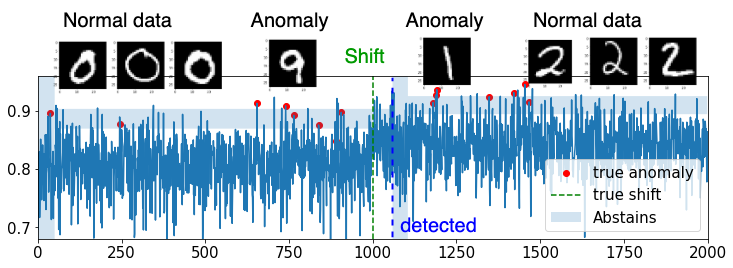
\includegraphics[width=0.9\linewidth]{anomaly/figs/Diagram2.png}
    \caption{MNIST experiment setup and a sample stream of (NN+A5) result. We choose a different set of digits for normal and anomaly to create the distribution shift, which our algorithm detects with a small delay. }
    \label{fig:mnist}
\end{figure}

\subsection{Case study of real AD application}

We also perform a case study on two real world datasets ({\ttfamily DS1} and {\ttfamily DS2}) obtained from large scale cloud computing services. Each dataset is a stream of anomaly scores obtained by applying the same black box anomaly detection algorithm (Details in Table \ref{tab:real_data_stats}). The practically motivated target in these datasets is to report $0.001\%$ anomalies, i.e., $p = 1-10^{-6}$.
Table \ref{tab:real_data} in the appendix reports the full result and comparison to baselines. We found that {\em(i)} our method achieves desired anomaly volume, {\em(ii)} incorporating offline data reduces the number of abstains without changing the volume of anomalies raised, and {\em(iii)} the volume of anomalies detected by all other methods are an order of magnitude higher leading to alert-fatigue. 
